\documentclass[11pt]{amsbook}

\usepackage[english,turkish]{babel}
\usepackage{../HBSuerDemir}	% ------------------------

\usepackage{fancyhdr} % Header/Footer
\pagestyle{fancy}
\thispagestyle{fancy}
\fancyhf{}
% \fancyhead[L]{\rightmark} %use this for autoshowing section name
\lhead{1. BÖLÜM}
\fancyfoot[L]{\footnotesize 
	Çizge Kuramı by Ceyhun  \textbf{DRAFT} \\
	\LaTeX ~by Haluk Bingol 
	\href{http://www.cmpe.boun.edu.tr/~bingol}
	{http://www.cmpe.boun.edu.tr/bingol} 
	%\large 
	%\footnotesize 
	\today}
\fancyfoot[R]{{\thepage} of \pageref{LastPage}}

\begin{document}
	
	% ++++++++++++++++++++++++++++++++++++++
	\hPage{ceyhun/23}
	% ++++++++++++++++++++++++++++++++++++++
	\bigskip\\\\
	$d_j$ nin kertesi $d_m$ nin kertesinden büyük olduğu
	için, $d_j$ ye bitişik olan ama $d_m$ ye bitişik olmayan
	bir $d_n$ düğümü vardır (Şekil~\ref{fig:1.3.2a}). 
	$\Large\c{C}$ den ($d_i$,$d_m$) ve ($d_j$,$d_n$)
	ayrıtları çıkarılıp yerine ($d_i$,$d_j$) ve ($d_m$,$d_n$)
	ayrıtlarının eklenmesi ile elde edilen $\Large\c{C}^\prime$
	çizgesinin kerte dizisi, $\Large\c{C}$ nin kerte dizisine özdeştir
	(Şekil~\ref{fig:1.3.2b}).
	\\\\
	\begin{figure}[h]
		\centering
		\subfigure[]{
			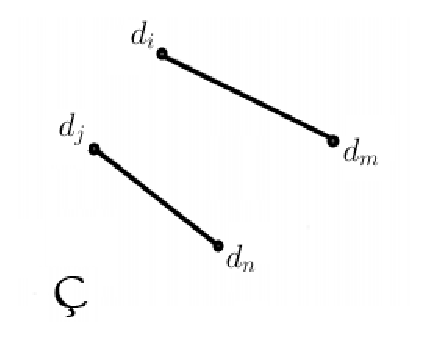
\includegraphics[width=.4\linewidth]{images/ceyhun-23-1-3-2a.eps}
			\label{fig:1.3.2a}
		}
		\quad
		\subfigure[]{
			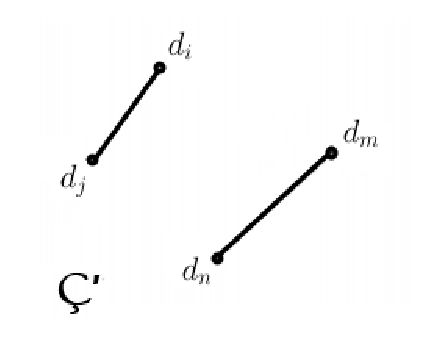
\includegraphics[width=.4\linewidth]{images/ceyhun-23-1-3-2b.eps}
			\label{fig:1.3.2b}
		}
		\label{fig:1.3.2}
		\caption{Teorem 1.3.1, Durum 2'de gerek koşulun açıklanması}
	\end{figure}
	
	\bigskip\noindent\\
	Öyleyse, yukarıda açıkladığımız bu ayrıtların yerdeğiştirme işlemi
	yeterince yinelenerek, Durum 1'deki koşulu sağlayan bir çizge her 
	zaman elde edilecektir.
	\\\\
	Verilen tamsayılar dizisini, eğer olanağı varsa, bir çizge ile 
	gerçekleştirmek için Teorem 1.3.1'den
	
	% =======================================================
\end{document}  